\documentclass[11pt]{article}
\usepackage{fullpage}
\usepackage{amsmath, amsfonts}
\usepackage[utf8]{inputenc}

\usepackage{graphicx}
\graphicspath{ {images/} }

\begin{document}
\begin{center}
{{\Large \sc Introduction to Machine Learning and Data Mining}}
\end{center}
\rule{\textwidth}{1pt}
\begin{description}
\item[Student names and ids:] Anders H. Opstrup (s160148); Gu Jinshan (s161944)
\item[Report:] 1
\end{description}
\rule{\textwidth}{1pt}

% 1. Description of our data set.
\section{Description of the data set}
This section of the report will shed some light on basic information about the dataset used in the project. The dataset is a collection of forest fires. The goal of the data is to try to predict forest fries in an attempt to prevent casualties and property damages. A further description of the attributes in the dataset can be found in detailed explanation section of the report.

\subsection{Place of data}
The data is obtained from this link: http://archive.ics.uci.edu/ml/datasets/Forest+Fires

\subsection{Previously work on the data set}
P. Cortez and A. Morais. A Data Mining Approach to Predict Forest Fires using Meteorological Data.
In Proceedings of the 13th EPIA 2007 - Portuguese Conference on Artificial Intelligence, 
December, 2007. (http://www.dsi.uminho.pt/~pcortez/fires.pdf) \newline

In the above reference, the output "area" was first transformed with a ln(x+1) function.
Then, several Data Mining methods were applied. After fitting the models, the outputs were
post-processed with the inverse of the ln(x+1) transform. Four different input setups were
used. The experiments were conducted using a 10-fold (cross-validation) x 30 runs. Two
regression metrics were measured: MAD and RMSE. A Gaussian support vector machine (SVM) fed
with only 4 direct weather conditions (temp, RH, wind and rain) obtained the best MAD value:
12.71 +- 0.01 (mean and confidence interval within 95\% using a t-student distribution). The
best RMSE was attained by the naive mean predictor. An analysis to the regression error curve
(REC) shows that the SVM model predicts more examples within a lower admitted error. In effect,
the SVM model predicts better small fires, which are the majority.

\subsection{Primary machine learning modeling aim}
Detection and test of outlier methods and try different regression methods and look at the correlation between the temperature, wind, rain and the burn area. 


% 2. Detailed explanation of the attributes of the data.
\begin{itemize}
\item \textbf{Describe if the attributes are discrete/continous, Nominal/Ordinal/Interval/Ratio.}
	\begin{enumerate}
	\item X - Discrete, Nominal
	\item Y - Discrete, Nominal
	\item month - Discrete, Ordinal
	\item day - Discrete, Ordinal
	\item FFMC - Continous, Interval
	\item DMC - Continous, Interval
	\item DC - Continous, Interval
	\item ISI - Continous, Interval
	\item temp - Continous, Interval
	\item RH - Continous, Ratio
	\item wind - Continous, Ratio
	\item rain - Continous, Ratio
	\item area - Continous, Ratio
	\end{enumerate}
\item \textbf{Give an account of whether there are data issues (i.e. missing values or corrupted data) and describe them if so.}\\
There is no missing values or corrupted data.
\item \textbf{Describe the basic summary statistics of the attributes.}\\
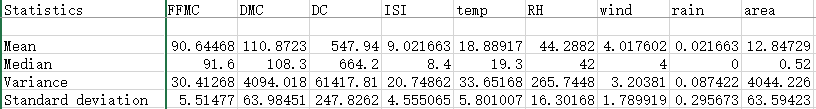
\includegraphics[width=\textwidth]{summary_statistics.png}
\end{itemize}
	

% 3. Data visualization(s) based on suitable visualization techniques in- cluding a principal component analysis (PCA).

% 4. Discussion explaining what we have learned about the data.

\end{document}